\section{Quality vs output length}
\label{app:quality}

The diffusion model degrades gracefully against a \emph{time} budget
and catastrophically against an \emph{output-length} budget. At
$L{=}128$ the AR model retains \arFOneTwentyEight{} F1 and
\arValidTwentyEight\% schema validity, while the diffusion model falls
to \dgFOneTwentyEight{} and \dgValidTwentyEight\%. Which budget an
application faces decides which architecture is safer.

\begin{figure}[t]
\centering
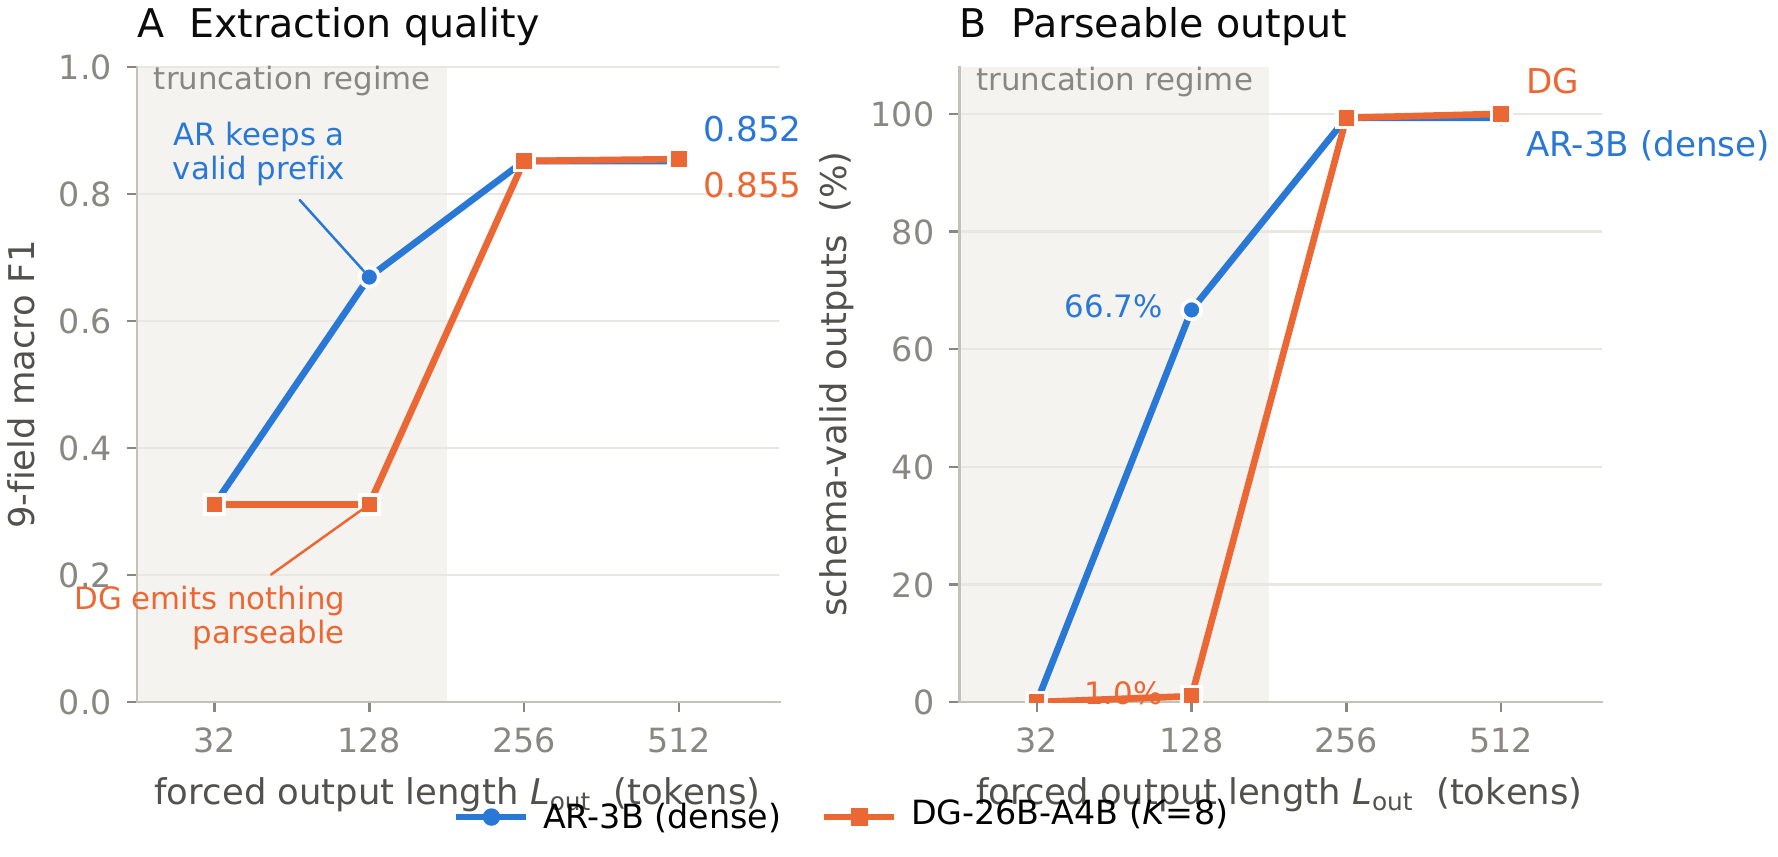
\includegraphics[width=\linewidth]{figures/fig5_quality_vs_length_hires.png}
\caption{Quality and schema validity vs forced output length (BGL,
$n{=}300$; AR arm is dense AR-3B). The diffusion model's quality rises
with $L$ and plateaus; AR-3B F1 is flat from $L{=}256$ to $L{=}512$
because first-object-wins parsing discards the rambled continuation.}
\label{fig:quality}
\end{figure}
